\begin{frame}[fragile]{Block Header}
  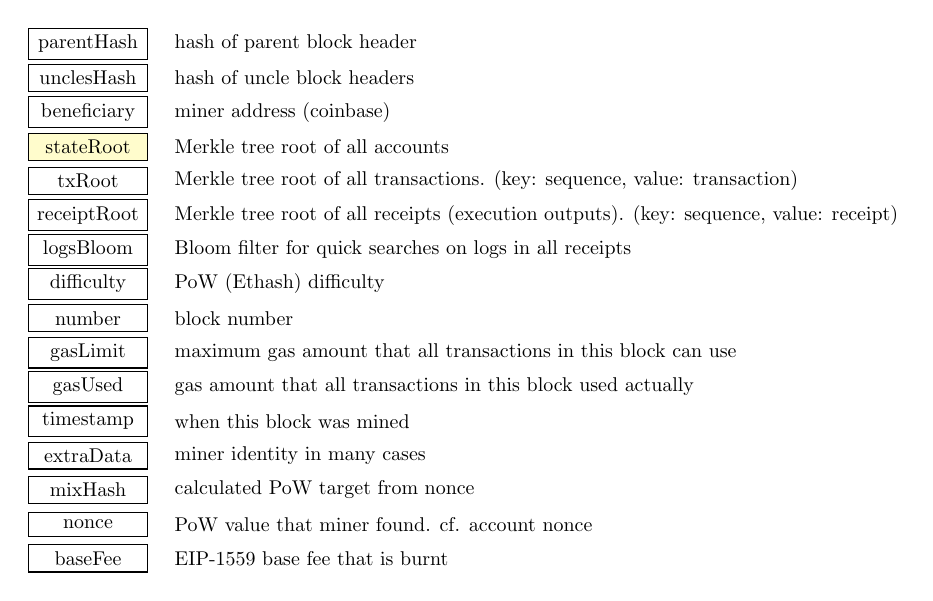
\begin{tikzpicture}[scale=0.72,every node/.style={transform shape}]
    \tikzstyle{field}=[minimum width=6em,minimum height=2.8ex,draw]
    \tikzstyle{desc}=[right=+4em]
    \node[field] at (0,0) {parentHash};
      \node[desc] at (0,0) {hash of parent block header};
    \node[field] at (0,-4ex) {unclesHash};
      \node[desc] at (0,-4ex) {hash of uncle block headers};
    \node[field] at (0,-8ex) {beneficiary};
      \node[desc] at (0,-8ex) {miner address (coinbase)};
    \node[field,fill=yellow,fill opacity=0.2,text opacity=1.0] at (0,-12ex) {stateRoot};
      \node[desc] at (0,-12ex) {Merkle tree root of all accounts};
    \node[field] at (0,-16ex) {txRoot};
      \node[desc] at (0,-16ex) {Merkle tree root of all transactions. (key: sequence, value: transaction)};
    \node[field] at (0,-20ex) {receiptRoot};
      \node[desc] at (0,-20ex) {Merkle tree root of all receipts (execution outputs). (key: sequence, value: receipt)};
    \node[field] at (0,-24ex) {logsBloom};
      \node[desc] at (0,-24ex) {Bloom filter for quick searches on logs in all receipts};
    \node[field] at (0,-28ex) {difficulty};
      \node[desc] at (0,-28ex) {PoW (Ethash) difficulty};
    \node[field] at (0,-32ex) {number};
      \node[desc] at (0,-32ex) {block number};
    \node[field] at (0,-36ex) {gasLimit};
      \node[desc] at (0,-36ex) {maximum gas amount that all transactions in this block can use};
    \node[field] at (0,-40ex) {gasUsed};
      \node[desc] at (0,-40ex) {gas amount that all transactions in this block used actually};
    \node[field] at (0,-44ex) {timestamp};
      \node[desc] at (0,-44ex) {when this block was mined};
    \node[field] at (0,-48ex) {extraData};
      \node[desc] at (0,-48ex) {miner identity in many cases};
    \node[field] at (0,-52ex) {mixHash};
      \node[desc] at (0,-52ex) {calculated PoW target from nonce};
    \node[field] at (0,-56ex) {nonce};
      \node[desc] at (0,-56ex) {PoW value that miner found. cf. account nonce};
    \node[field] at (0,-60ex) {baseFee};
      \node[desc] at (0,-60ex) {EIP-1559 base fee that is burnt};
  \end{tikzpicture}
\end{frame}